%
% drehung.tex -- Drehungen
%
% (c) 2020 Prof Dr Andreas Müller, Hochschule Rapperswil
%
% !TEX root = ../../buch.tex
% !TEX encoding = UTF-8
%

\section{Drehungen\label{qa:section:drehungen}}
\kopfrechts{Drehungen}
\subsection{Eulersche Formel}
Bevor Drehungen durchgeführt werden können, muss klargestellt werden, 
wie die vier Dimensionen verwendet werden: Die imaginären Achsen 
$i,j,k$ werden den drei Raumachsen $x,y,z$ zugeordnet. Damit kann eine 
Drehung um die $x$-Achse um 90°mit der Quaternion $0 + 1i + 0j + 0k$ 
durchgeführt werden. Analog dazu kann eine Drehung um die $y$-Achse 
mit der Quaternion $0 + 0i + 1j + 0k$ und eine Drehung um die 
$z$-Achse mit der Quaternion $0 + 0i + 0j + 1k$ durchgeführt werden.

Der Realteil gibt den Winkel der 
Drehung an. Dafür wird die eulersche Drehformel in der Form
\begin{equation*}
    e^{i\vartheta} = \cos(\vartheta) + i\sin(\vartheta)
\end{equation*}
verwendet, welche bei den komplexen Zahlen eine Drehung um $\vartheta$ 
beim Nullpunkt in der komplexen Ebene beschreibt. Für Quaternionen 
wird die Formel erweitert, sodass eine Drehung um eine beliebige 
Achse durchgeführt werden kann. Die Achse wird durch einen 
Einheitsvektor beschrieben, welcher die Richtung der Achse angibt. 
Der Winkel $\vartheta$ gibt, gleich wie bei den komplexen Zahlen, 
das Ausmass der Drehung an. Damit kann eine Quaternion für eine 
Drehung um eine beliebige Achse mit der Formel
\begin{equation*}
    q = e^{\vartheta(xi + yj + zk)} 
    = \cos \left(\vartheta\right) 
    + \frac{xi + yj + zk}{\sqrt{x^2 + y^2 + z^2}}\sin\left(\vartheta\right)
\end{equation*}
berechnet werden. Der Bruch vor dem Sinus-Term stellt sicher, dass 
der Imaginärteil der Quaternion ein Einheitsvektor ist. Die Formel 
ist jedoch in dieser Form noch nicht anwendbar, wie im nächsten 
Beispiel gezeigt wird.

\begin{beispiel}
    Sei ein Punkt $P_1$ auf der $z$-Achse mit den Koordinaten $(0,0,1)
    $. Mit Quaternionen lässt sich $P_1$ wie folgt darstellen: $P_1 = 0
    + 0i + 0j + 1k$. Dieser Punkt soll um die $z$-Achse um 90° (oder 
    $\frac{\pi}{2}$) gedreht werden. Das erwartete Ergebnis ist 
    wiederum $(0,0,1)$, da eine Drehung um die eigene Achse keine 
    Wirkung hat. Die Quaternion für diese Drehung wird mit 
    \begin{equation*}
        q = e^{\frac{\pi}{2}(0i + 0j + 1k)} 
        = \cos\left(\frac{\pi}{2}\right) 
        + \frac{0i + 0j + 1k}{|0 + 0 + 1|}
        \sin\left(\frac{\pi}{2}\right) 
        = k
    \end{equation*}
    berechnet. Nun soll die Drehung durchgeführt werden. Dafür wird die 
    Quaternion $q$ von links her mit dem Punkt $P_1$ multipliziert, was
    \begin{equation*}
        P_{1L} = q \cdot P_1 = k \cdot k = k^2 = -1
    \end{equation*}
    ergibt.
    Das Ergebnis ist $-1$, was dem Punkt $(0,0,0)$ mit Realteil $-1$ entspricht. 
    Statt dass der Punkt auf der $z$-Achse geblieben ist, wurde er weder Erwarten 
    auf den Ursprung verschoben mit Länge 1 in der vierten Dimension.
\end{beispiel}

\subsubsection{Visualisierung}
%
% videoqrcode.tex
%
% (c) 2026 Prof Dr Andreas Müller
%
\vspace*{-12pt}
\smash{\hbox to\hsize{\hfill\raisebox{-1.2cm}{%
\qrcode[height=1.6cm]{https://youtu.be/7kv7XFGp4ns}%
}}}%
\hangindent=-2.1cm
\hangafter=-6

Vierdimensionale Zahlen lassen sich nicht leicht visualisieren. 
Eine Möglichkeit ist, die imaginären Achsen in einem 
dreidimensionalen Koordinatensystem und die vierte Dimension 
zusammen mit der $z$-Achse in einem zweidimensionalen 
Koordinatensystem darzustellen. Abbildung \ref{qa:fig:Drehung} zeigt in vier 
Schritten die Drehung des vorherigen Beispiels. Zusätzlich wurde ein Würfel mit 
den Kantenlängen $1$ in das Koordinatensystem eingefügt, um das Verhalten des Raumes 
zu verdeutlichen.
Alternativ kann die Animation zu dieser Drehung über den beiliegenden QR Code abgespielt werden.

\begin{figure}
    \centering
    \begin{minipage}{0.48\textwidth}
        \centering
        \subfigure[Ausgangslage]{%
            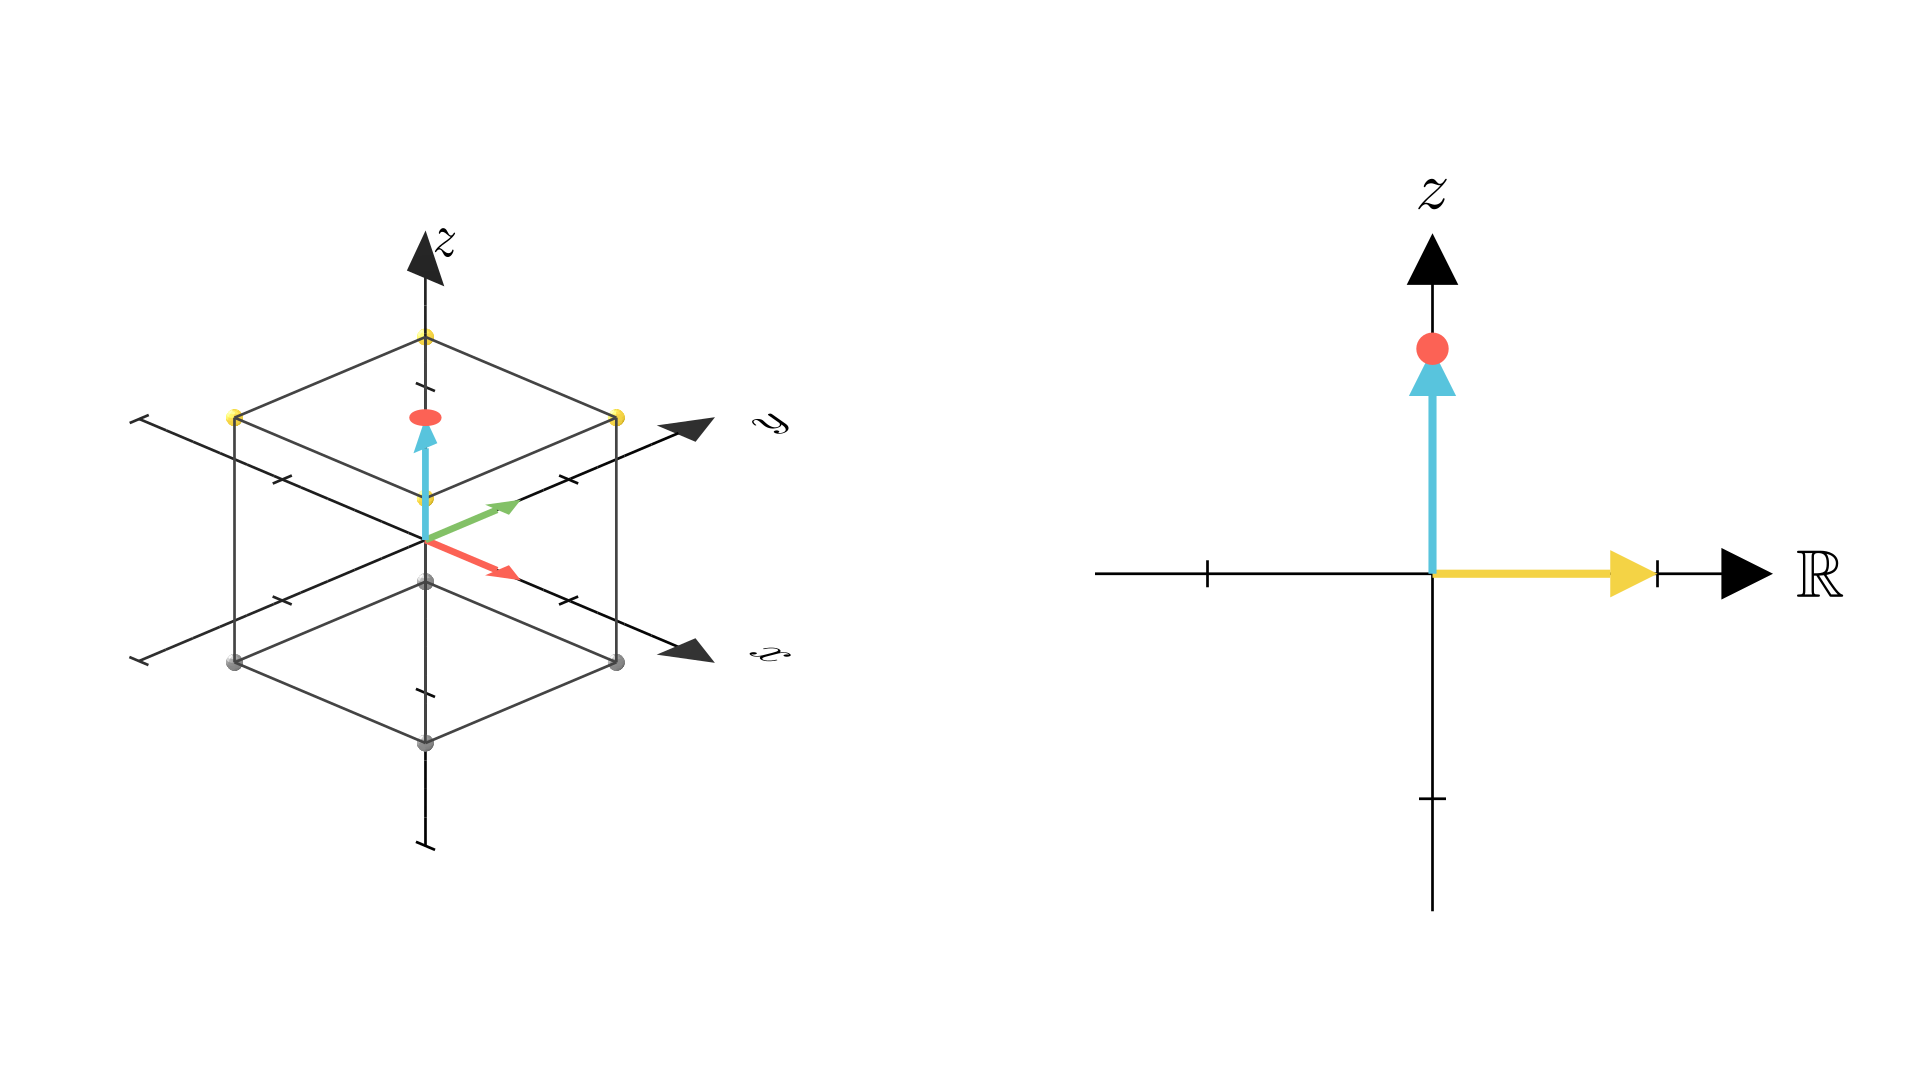
\includegraphics[width=\textwidth,trim=80 160 40 130,clip]{papers/qa/img/Quaternion_rot_1.png}}
    \end{minipage}
    \hfill
    \begin{minipage}{0.48\textwidth}
        \centering
        \subfigure[Beginn der Drehung]{%
            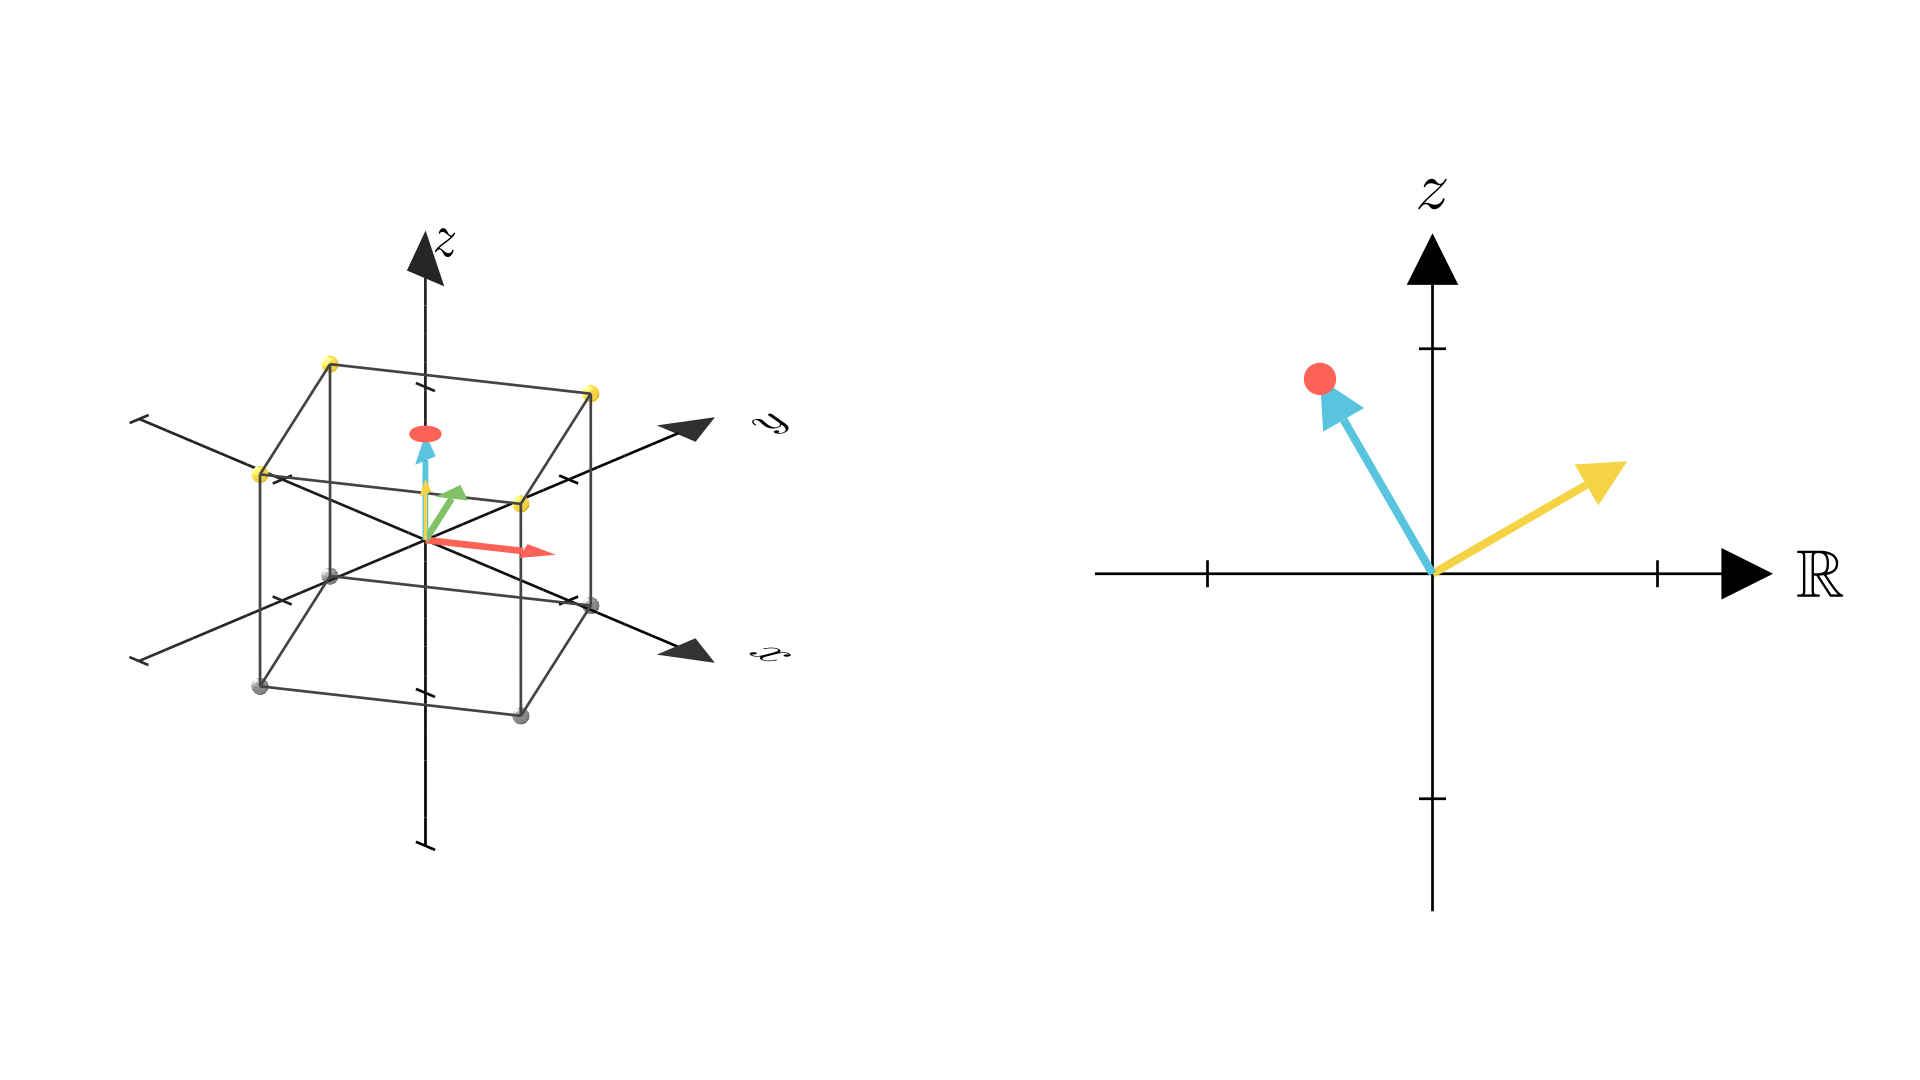
\includegraphics[width=\textwidth,trim=80 160 40 130,clip]{papers/qa/img/Quaternion_rot_2.png}}
    \end{minipage}

    \vspace{1em}

    \begin{minipage}{0.48\textwidth}
        \centering
        \subfigure[Fortgeschrittene Drehung]{%
            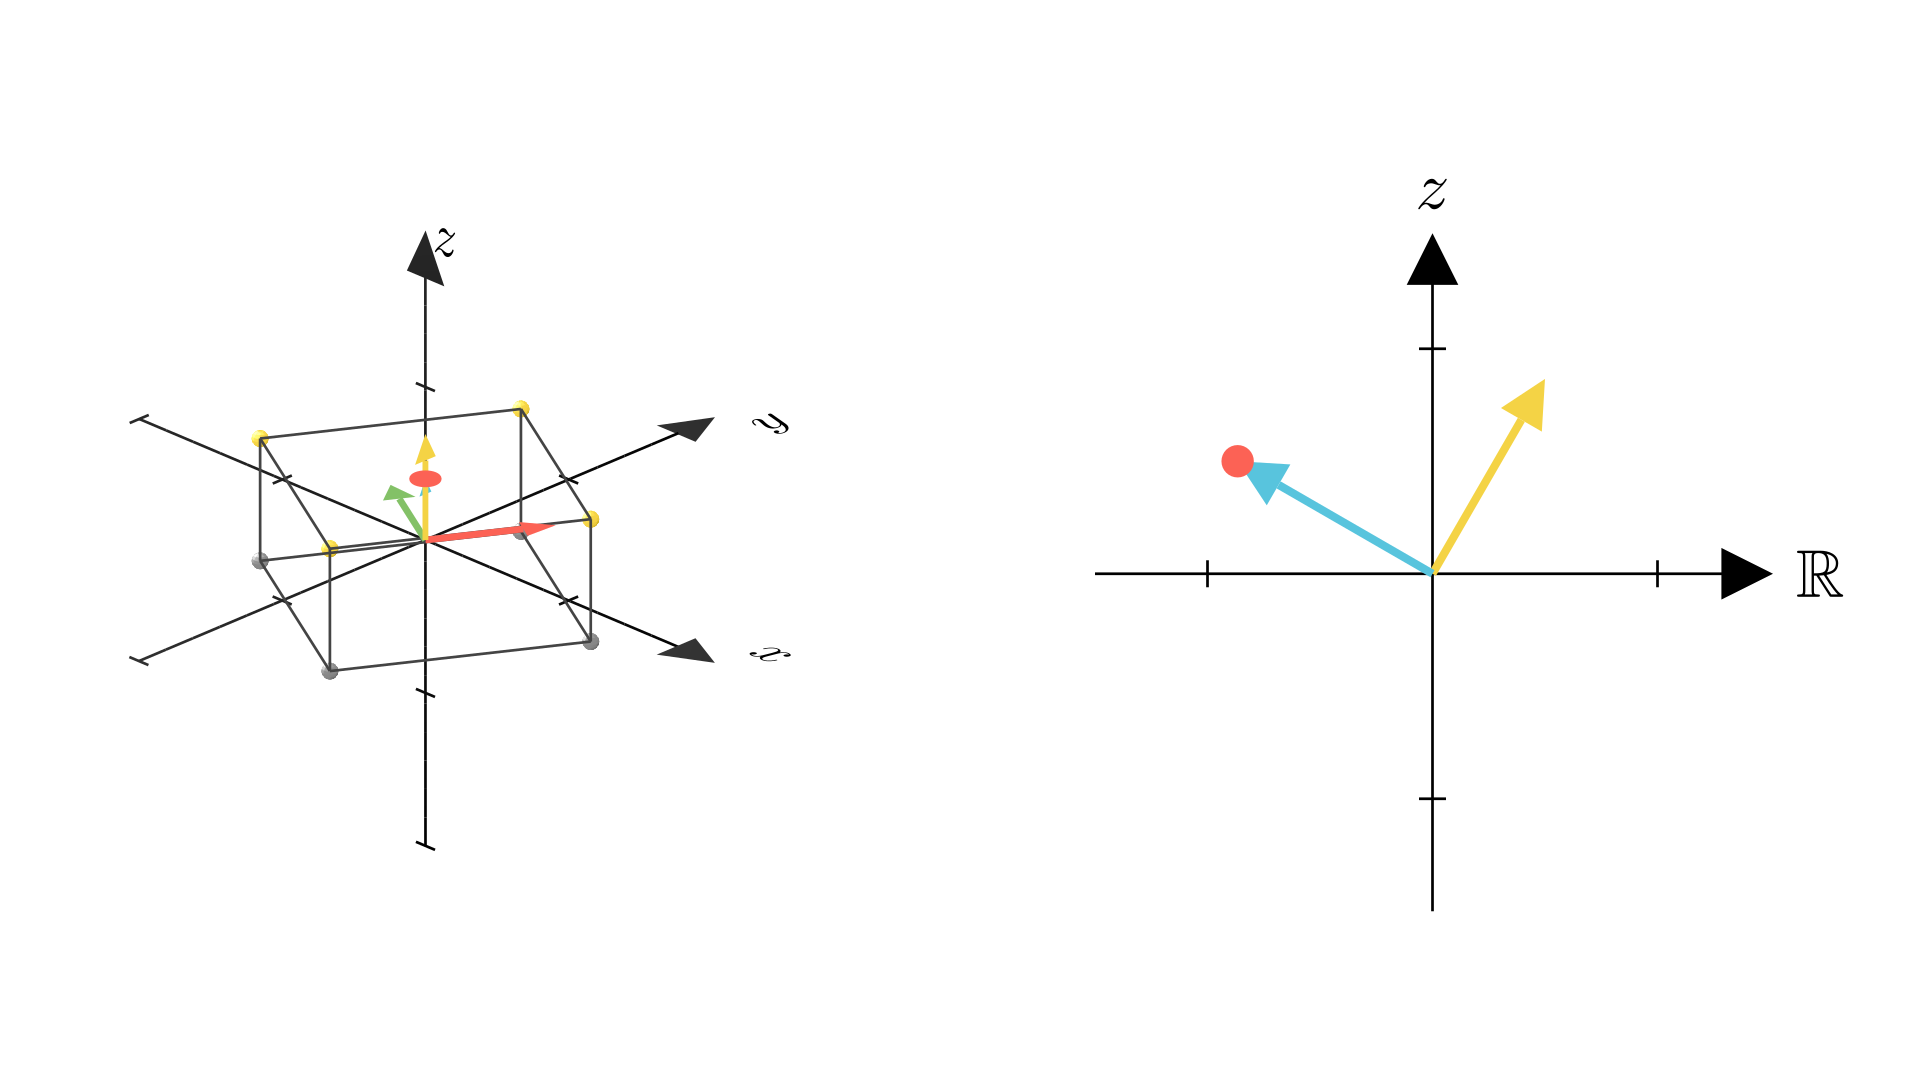
\includegraphics[width=\textwidth,trim=80 160 40 130,clip]{papers/qa/img/Quaternion_rot_3.png}}
    \end{minipage}
    \hfill
    \begin{minipage}{0.48\textwidth}
        \centering
        \subfigure[Endlage]{%
            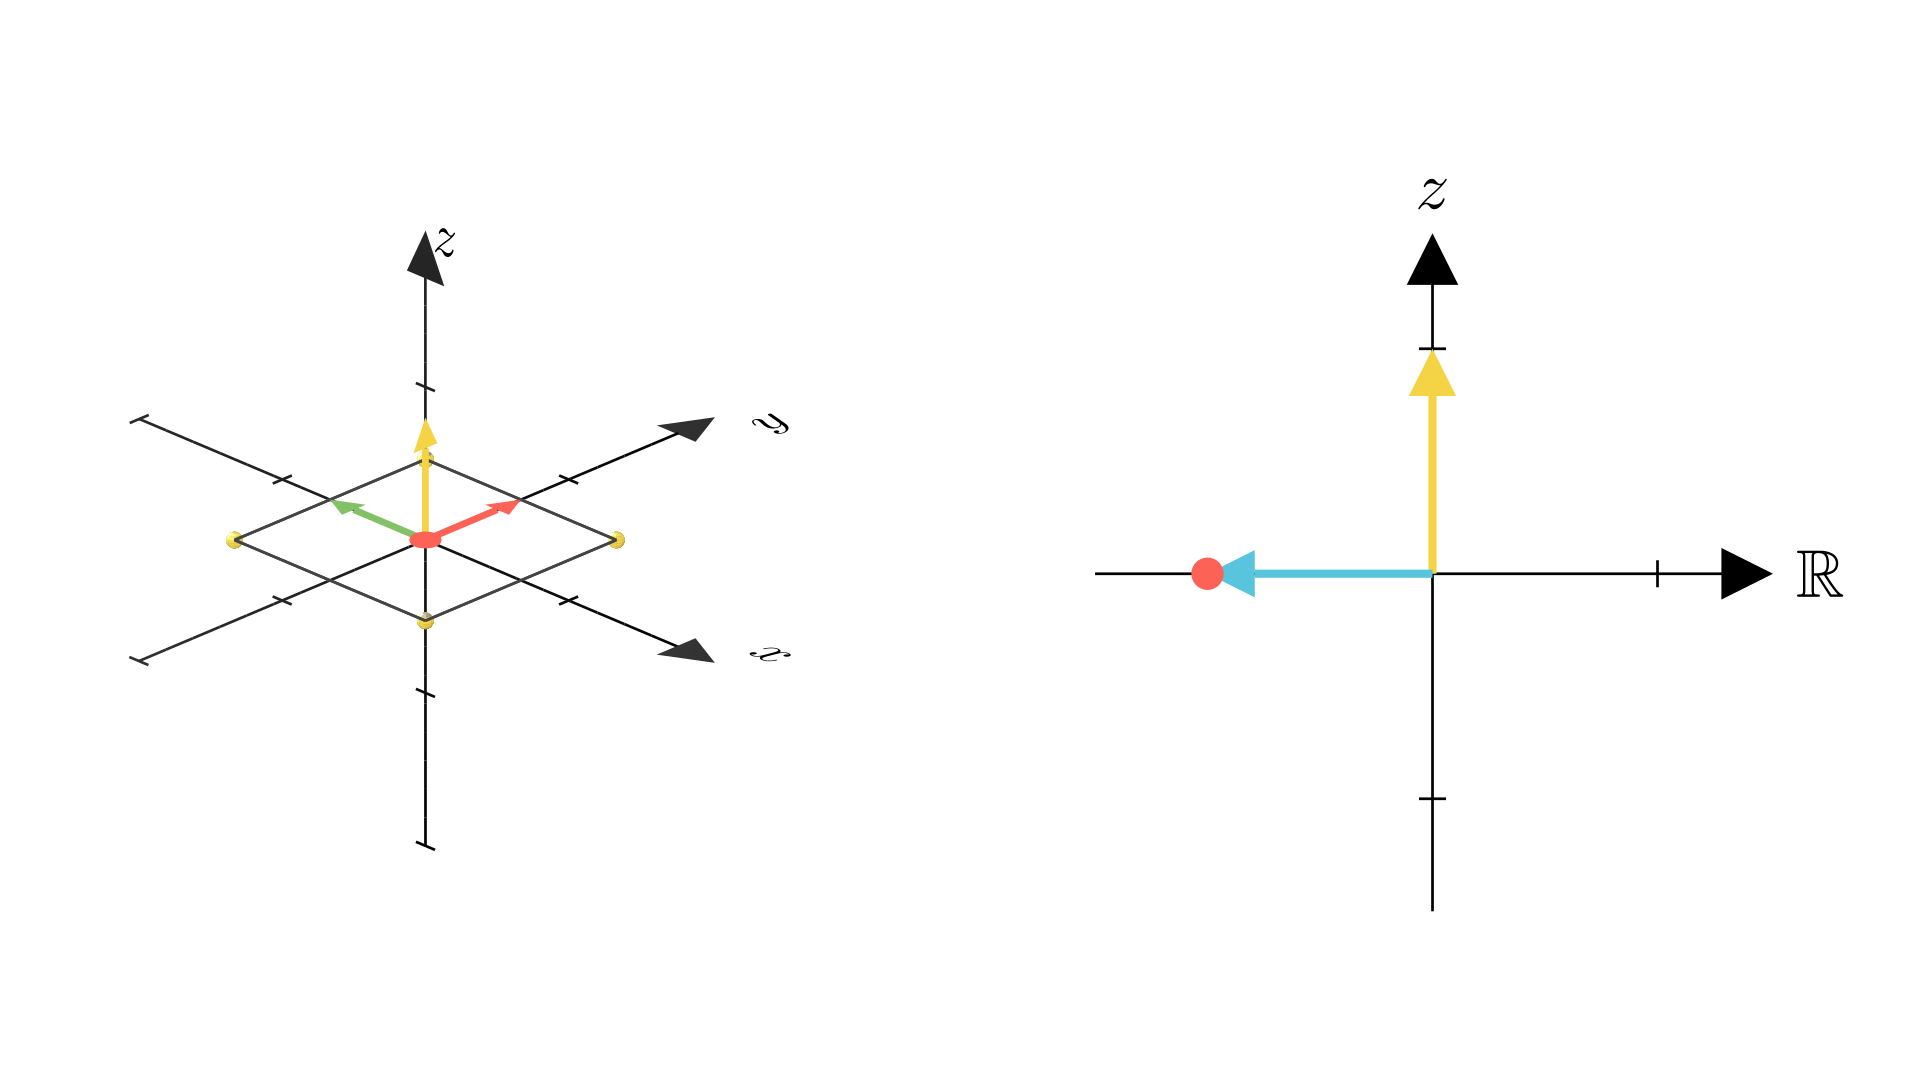
\includegraphics[width=\textwidth,trim=80 160 40 130,clip]{papers/qa/img/Quaternion_rot_4.png}}
    \end{minipage}
    \caption{Visualisierung der Multiplikation $P_{1L} = q \cdot P_1$ mit
    $q = k$. In der Ausgangslage zeigen der rote, grüne und blaue Pfeil 
    im dreidimensionalen koordinatensystem auf die $x,y,z$-Achsen und 
    repräsentieren die imaginären $i,j,k$-Achsen,
    während der gelbe Pfeil im zweidimensionalen Koordinatensystem in die 
    reelle Achse zeigt. Der gelbe Pfeil steht orthogonal zu allen anderen 
    Pfeilen, in der vierten Dimension. Der rot markierte Punkt $P_1$ liegt 
    auf $(1,0,0)$. Schritt für Schritt wird der Punkt um 90° um die 
    $z$-Achse gedreht, bis er in der Endlage auf $(0,0,0)$ liegt. Dabei 
    bewirkt die Multiplikation die Verschiebung des Punktes in die vierte 
    Dimension, sodass der Punkt nicht mehr im dreidimensionalen Raum liegt.}
    \label{qa:fig:Drehung}
\end{figure}

Der rote, grüne und blaue Pfeil in den Bildern zeigt jeweils in 
die $x,y,z$-Achsen und repräsentieren die imaginären $i,j,k$-Achsen. 
Der gelbe Pfeil zeigt in die reele Achse und ist orthogonal zu 
allen anderen Achsen. In anderen Worten: Man muss sich vorstellen, 
dass der gelbe Pfeil rechtwinklig steht zu allen anderen Pfeilen, 
in der vierten Dimension. Der rot markierte Punkt $P_1$ liegt nun im 
Ursprung, mit $-1$ in der reellen Achse.

\subsubsection{Multiplikation von Rechts}

Um den Punkt tatsächlich um 90° um die $z$-Achse im 
Gegenuhrzeigersinn zu drehen, muss die Rolle der Reihenfolge 
analysiert werden. Dafür wird ein neuer Beispielpunkt $P_2 = (0,1,1)
$ verwendet, welcher nach einer Drehung auch den Ort wechselt. Eine 
Multiplikation von Links würde
\begin{equation*}
    P_{2L} = q P_2 
    = k \cdot (0 + 0i + 1j + 1k) 
    = k (j + k) 
    = kj + k^2 
    = -i - 1
\end{equation*}
ergeben, was dem Punkt $(-1,0,0)$ im 3D-Raum entspricht. Der 
Punkt wurde also um 90° um die $z$-Achse im Gegenuhrzeigersinn 
gedreht, jedoch wurde der $z$-Anteil des Punktes auf 0 reduziert. 
Der Realteil beträgt $-1$.

Von Rechts würde die Multiplikation
\begin{equation*}
    P_{2R} 
    = P_2 q 
    = (0 + 0i + 1j + 1k) k 
    = jk + k^2 
    = i - 1
\end{equation*}
lauten, was dem Punkt $(1,0,0)$ entspricht. Von Rechts wurde 
der Punkt also um 90° in umgekehrter Drehrichtung um die $z$-Achse 
gedreht. Auch hier wurde der $z$-Anteil des Punktes auf 0 
reduziert, mit Realteil $-1$.

Die Multiplikation von Links und Rechts betrifft also primär die 
Richtung der Drehung. Es ist zu beachten, dass für beide 
Multiplikationen das selbe Phänomen auftritt, dass der $z$-Anteil 
des Punktes auf 0 reduziert und der Realteil auf $-1$ gesetzt wird. 
Anders ausgedrückt: Die entstandene Verzerrung ist sowohl bei 
Linksmultiplikation als auch bei Rechtsmultiplikation identisch. 
Im nächsten Abschnitt wird gezeigt, wie dieser Nebeneffekt elegant 
gelöst werden kann.
\subsection{Die Drehformel\label{qa:section:drehungen:drehformel}}%
Für die effektive Drehung werden die folgenden Eigenschaften der 
Quaternionen verwendet:
\begin{itemize}
    \item Multiplikation von Links: Gegenuhrzeigersinn mit 
''Realteil''
    \item Multiplikation von Rechts: Uhrzeigersinn mit identischem ''Realteil''
    \item Inverse einer Quaternion: $q^{-1}$ macht die Drehung 
    rückgängig, sodass $q q^{-1} = 1$
    \item Bei Einheitsquaternionen gilt: $q^{-1} = q^*$, wobei $q^*$ 
    die konjugierte Quaternion ist
\end{itemize}
Für die verzerrungsfreie Drehung wird zuerst der Punkt $P$ mit der 
Quaternion $q$ von Links multipliziert, was in unserem Beispiel 
eine Drehung um 90° im Gegenuhrzeigersinn ergibt. Danach wird das 
Ergebnis von Rechts mit der Inverse desselben Quaternion $q^{-1}$ 
multipliziert, welches erneut eine Drehung um 90° im 
Gegenuhrzeigersinn bewirkt. Die Inverse hat dabei zwei 
entscheidende Wirkungen:
\begin{itemize}
    \item Die zweite Drehung macht die Verzerrung rückgängig
    \item Die Drehrichtung von Rechts wird umgekehrt, sodass zwei 
    aufeinanderfolgende Drehungen in gleicher Richtung erfolgen
\end{itemize}
Die Drehformel lautet also
\begin{equation*}
    P' = q P q^{-1}.
\end{equation*}
Und für Einheitsquaternionen kann die Formel auch in der Form
\begin{equation*}
    P' = q P q^*
\end{equation*}
geschrieben werden. Die Berechnung der Konjugation ist deutlich
einfacher als die Berechnung der Inversen, da nur die Vorzeichen
der Imaginärteile geändert werden müssen.
Mit dem Beispielpunkt $P_2$ und der Quaternion $q$ für eine Drehung
um 90° um die $z$-Achse ergibt sich
\begin{align*}
    P' &= q P_2 q^{-1} \\
    &= k (0 + 0i + 1j + 1k) k^{-1} \\
    &= k (j + k) (-k) \\
    &= kjk + kk(-k) \\
    &= -i - k^3 \\
    &= -i + k \\
    &= (-1, 0, 1) \quad \text{(ohne Realteil!)}.
\end{align*}
Es ist zu beachten, dass nun eine 180° Drehung durchgeführt wurde, 
da die Multiplikation von Links und Rechts jeweils eine 90° Drehung 
bewirkt. Das heisst, um eine Drehung um 90° zu erreichen, muss der 
Winkel $\vartheta$ in der Berechnung der Quaternion $q$ halbiert werden,
also $\vartheta = \frac{\pi}{4}$. Somit wird die Formel wie folgt umgestellt,
\begin{equation*}
    q = \cos\left(\frac{\vartheta}{2}\right) 
    + \frac{xi + yj + zk}{\sqrt{x^2 + y^2 + z^2}}
    \sin\left(\frac{\vartheta}{2}\right)
\end{equation*}
sodass der Punkt tatsächlich um den gewünschten Winkel $\vartheta$ gedreht wird.

